\section{HDR1軸力覚センサの設計}
\subsection{起歪体の構造}
提案する力覚センサの構造とひずみゲージ貼り付け位置をFig.~\ref{fig:sensor}に, 
起歪体の寸法をTable~\ref{tb:size}に示す.
本研究ではセンシング部分の提案によるHDRの原理的検証を目的としているため, 
起歪体の構造は非常に単純な片持ち梁を採用した. 
また, 大荷重に耐えられるよう起歪体の材料は剛性の高い超々ジュラルミンを採用した. 

\subsection{ひずみゲージ貼り付け位置}
有限要素法シミュレーションによる起歪体のひずみ分布をFig.~\ref{fig:sim}に示す.

ひずみゲージは被測定対象のひずみが伝達することにより抵抗変化が生じる
センシング素子である. 
ひずみの変化は大変微小であるため, ひずみゲージの貼り付け位置は
測定対象のよりひずみやすい部分に貼り付けることが求められる. 
よって有限要素法シミュレーションにより任意の荷重を印加, 
この時のひずみ分布をもとに貼り付け位置を決定した. 
ひずみゲージは$F_z$方向の荷重を受けた時にひずむ面に表裏合わせて二枚貼り付けた. 
また, このシミュレーション結果より得られた本センサの定格荷重と
定格荷重印加時の安全率のパラメータをTable~\ref{tb:kajuu}に示す.
\begin{table}[h]
  \caption{起歪体の寸法 [mm]\\Table. 2 Dimensions of strain body [mm]}\label{tb:size}
  \begin{center}
   \begin{tabular}{ c c c c }
    \hline
     & Length & Width & Height  \\
    \hline
    Cantilever beam & 100 & 10 & 10  \\
    \hline   
   \end{tabular}
  \end{center}
 \end{table}
\begin{table}[h]
  \caption{定格荷重と安全率\\Table. 3 Rated load and safety factor}\label{tb:kajuu}
  \begin{center}
   \begin{tabular}{ c c }
    \hline
    定格荷重 $F$[N] & 安全率 \\
    \hline
    200.0 & 1.145 \\
    \hline   
   \end{tabular}
  \end{center}
 \end{table}

\begin{figure}[h]
  \centering
  \begin{tabular}{c}
    \begin{minipage}{0.5\hsize}
      \begin{center}
        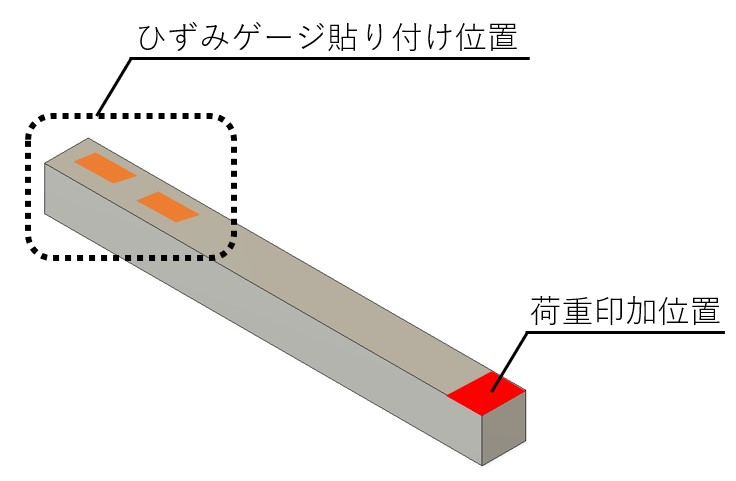
\includegraphics[scale=0.2]{pic/hari.jpg}
        \hspace{1.cm} 
        \footnotesize{起歪体\\Strain body}
      \end{center}
    \end{minipage}
        \begin{minipage}{0.51\hsize}
      \begin{center}
        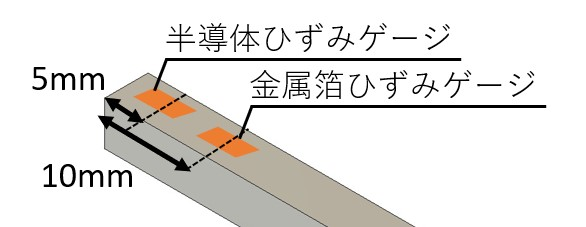
\includegraphics[scale=0.28]{pic/hizumi.jpg}
        \hspace{1.6cm} 
        \footnotesize{ひずみゲージの貼付位置\\Strain gauge application position}
      \end{center}
    \end{minipage}
  \end{tabular}
  \caption[]{HDR1軸力覚センサ\\Fig. 1 HDR unaxial force sensor}\label{fig:sensor}
\end{figure}

\begin{figure}[h]
  \begin{center}
    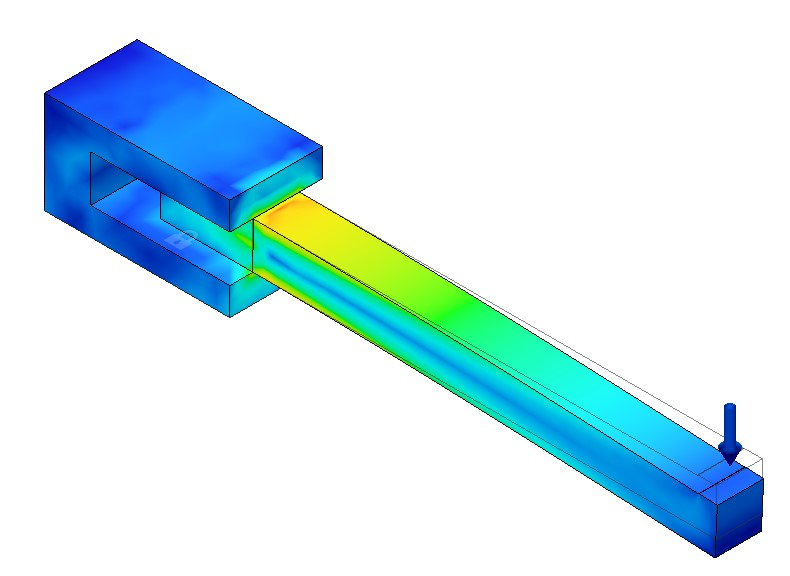
\includegraphics[width=5.2cm]{pic/simHizumi.jpg}
    \caption{ひずみ分布\\Fig. 2 Strain distribution}\label{fig:sim}
  \end{center}
\end{figure}

\subsection{測定回路系の構成と計測レンジ}
ひずみを取得するための測定回路をFig.~\ref{fig:sokuteikairo}
に示す. 
ひずみの変化を受けて抵抗値が変位するひずみゲージは, 
ホイートストンブリッジ回路に接続される. 
ブリッジ電圧を読み取り, A/D変換された値がカットオフ周波数$fc = 10$HzのLPFを通って
USB接続されたPCに出力されることで, ひずみの計測が行える. 
\begin{figure}[h]
  \begin{center}
    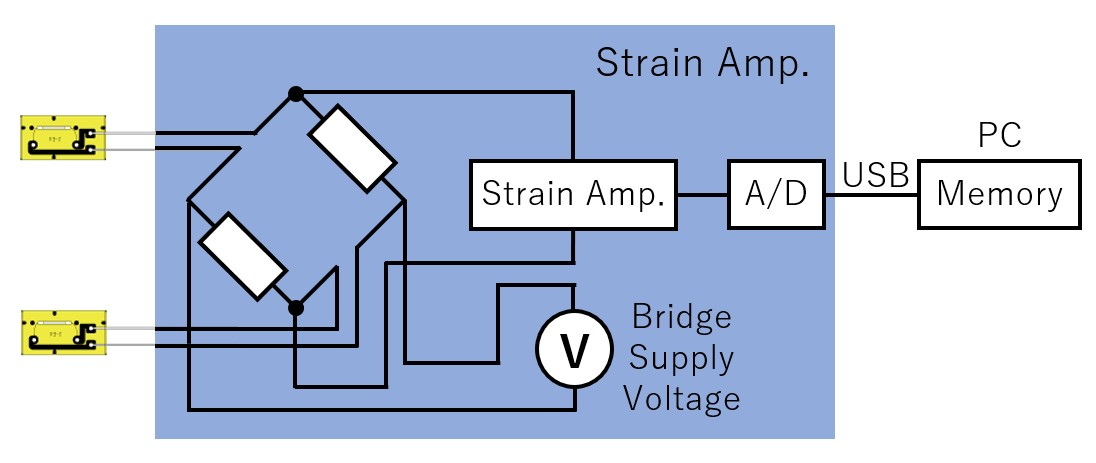
\includegraphics[width=7.5cm]{pic/sokuteikairo.jpg}
    \caption{測定回路\\Fig. 3 Measurement circuit}\label{fig:sokuteikairo}
  \end{center}
\end{figure}
\begin{figure}[h]
  \begin{center}
    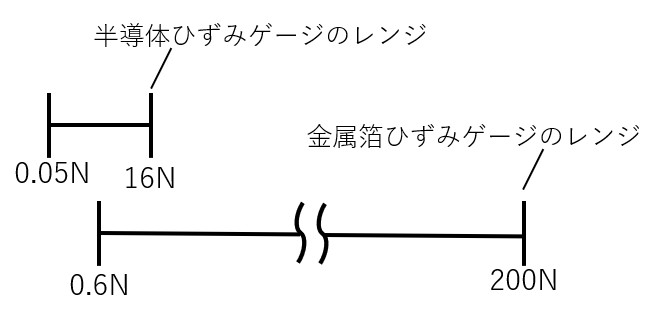
\includegraphics[width=7.5cm]{pic/range.jpg}
    \caption{各ひずみゲージの測定レンジ\\Fig. 4 Measurement range of each strain gauge}\label{fig:range}
  \end{center}
\end{figure}
ここで, 金属箔ひずみゲージと半導体ひずみゲージそれぞれの測定レンジを
Fig.~\ref{fig:range}に示す. 
今回使用したひずみアンプはPCD-400Aで, このひずみアンプの測定レンジは
最大$20000×10^{-6}$である. Table~\ref{tb:gage}に記したように
金属箔, 半導体ひずみゲージのひずみ限界はそれぞれ$20000, 3000×10^{-6}$であるが, 
出力として得られる値は, 起歪体に生じたひずみのゲージ率倍されたものである. 
よって, 金属箔ひずみゲージでは$10000×10^{-6}$までのひずみを出力として得ることができ, 
半導体ひずみゲージでは金属箔ひずみげーじでノイズに埋もれてしまう
低荷重域の値を$110×10^{-6}$まで出力値として得ることができる. 
このひずみのレンジを印加荷重のレンジに置き換えるとFig.~\ref{fig:range}
に示したレンジとなり, ゲージ率の異なるひずみゲージを併用することでHDRを
有した力覚センサを設計することが可能であると見込める. 

